% ICVSS poster format (70x90cm); landscape orientation is not allowed
\documentclass[ICVSS,portrait,final]{baposter}
% Generic poster format
%\documentclass[portrait,final]{baposter}
% a4shrink for an a4 sized paper (WARNING: aspect ratio of ICVSS posters is different from A4, may break layout)
%\documentclass[a4shrink,portrait,final]{baposter}

% ABOUT THIS TEMPLATE
% Poster template by Brian Amberg 2007
% Little changes and current ICVSS template by Eugenio Rustico 2010 (rustico@dmi.unict.it)
% Please do not mail us for general LaTeX questions. Thank you!
% Feel free to define new colors, change shape and layout of headerboxes.
% You can add an eyecatcher, set a background image, avoid drawing some headers (ghost option).
% About headerboxes: remember to define first the top and bottom ones.
%
% KNOWN ISSUES	
% - Something is wrong with some eyecatchers
% - Using pdftex breaks the page size [partially solved]

% Using pdftex (required by hyperref package) may lead to wrong page size.
% However, there is a workaround to import hyperref without breaking the
% page layout (thanks to Christian Nitschke for pointing it out).
% It is described here:
%   http://stackoverflow.com/questions/1496852/page-margins-change-in-pdflatex/1843929#1843929
% However, for some reasons background shading seems to be lost.
% To summarize: if you *really* need hyperref, choose a plain white background and
% uncomment the following:
% ---------------- FROM HERE
% \setlength{\paperwidth}{700mm}
% \setlength{\paperheight}{900mm}
% if PDFTeX
% % set commands \pdfpagewidth, \pdfpageheight which are only known to PDFTeX
% \ifx\pdfoutput\undefined
% \else
% \setlength{\pdfpagewidth}{\paperwidth}
% \setlength{\pdfpageheight}{\paperheight}
% \fi
% ---------------- TO HERE

\tracingstats=2

% Words in captital letters are marked as acronyms and hyphenated wrong.
% Let's tell LaTeX not to hyphen capitals at all
\uchyph=0

% Euro symbol
\usepackage{eurosym}
% hyperlinks
% can use hyperref (see above), but background shading may be lost (use plain white?)
%\usepackage[colorlinks=true,pdftex]{hyperref}
% urls
\usepackage{url}

\usepackage{times}
\usepackage{calc}
\usepackage{graphicx}
\usepackage{amsmath}
\usepackage{amssymb}
\usepackage{relsize}
\usepackage{multirow}
\usepackage{bm}

\usepackage{graphicx}
\usepackage{multicol}

\usepackage{pgfbaselayers}
\pgfdeclarelayer{background}
\pgfdeclarelayer{foreground}
\pgfsetlayers{background,main,foreground}

\usepackage{helvet}
%\usepackage{bookman}
\usepackage{palatino}

\newcommand{\captionfont}{\footnotesize}

\selectcolormodel{cmyk}

% all imgs in a subdir
\graphicspath{{images/}}

%%%%%%%%%%%%%%%%%%%%%%%%%%%%%%%%%%%%%%%%%%%%%%%%%%%%%%%%%%%%%%%%%%%%%%%%%%%%%%%%
%%%% Some math symbols used in the text
%%%%%%%%%%%%%%%%%%%%%%%%%%%%%%%%%%%%%%%%%%%%%%%%%%%%%%%%%%%%%%%%%%%%%%%%%%%%%%%%
% Format
\newcommand{\Matrix}[1]{\begin{bmatrix} #1 \end{bmatrix}}
\newcommand{\Vector}[1]{\Matrix{#1}}
\newcommand*{\SET}[1]  {\ensuremath{\mathcal{#1}}}
\newcommand*{\MAT}[1]  {\ensuremath{\mathbf{#1}}}
\newcommand*{\VEC}[1]  {\ensuremath{\bm{#1}}}
\newcommand*{\CONST}[1]{\ensuremath{\mathit{#1}}}
\newcommand*{\norm}[1]{\mathopen\| #1 \mathclose\|}% use instead of $\|x\|$
\newcommand*{\abs}[1]{\mathopen| #1 \mathclose|}% use instead of $\|x\|$
\newcommand*{\absLR}[1]{\left| #1 \right|}% use instead of $\|x\|$

\def\norm#1{\mathopen\| #1 \mathclose\|}% use instead of $\|x\|$
\newcommand{\normLR}[1]{\left\| #1 \right\|}% use instead of $\|x\|$

%%%%%%%%%%%%%%%%%%%%%%%%%%%%%%%%%%%%%%%%%%%%%%%%%%%%%%%%%%%%%%%%%%%%%%%%%%%%%%%%
% Multicol Settings
%%%%%%%%%%%%%%%%%%%%%%%%%%%%%%%%%%%%%%%%%%%%%%%%%%%%%%%%%%%%%%%%%%%%%%%%%%%%%%%%
\setlength{\columnsep}{0.7em}
\setlength{\columnseprule}{0mm}

%%%%%%%%%%%%%%%%%%%%%%%%%%%%%%%%%%%%%%%%%%%%%%%%%%%%%%%%%%%%%%%%%%%%%%%%%%%%%%%%
% Save space in lists. Use this after the opening of the list
%%%%%%%%%%%%%%%%%%%%%%%%%%%%%%%%%%%%%%%%%%%%%%%%%%%%%%%%%%%%%%%%%%%%%%%%%%%%%%%%
\newcommand{\compresslist}{%
\setlength{\itemsep}{1pt}%
\setlength{\parskip}{0pt}%
\setlength{\parsep}{0pt}%
}


%%%%%%%%%%%%%%%%%%%%%%%%%%%%%%%%%%%%%%%%%%%%%%%%%%%%%%%%%%%%%%%%%%%%%%%%%%%%%%
%%% Begin of Document
%%%%%%%%%%%%%%%%%%%%%%%%%%%%%%%%%%%%%%%%%%%%%%%%%%%%%%%%%%%%%%%%%%%%%%%%%%%%%%

\begin{document}

%%%%%%%%%%%%%%%%%%%%%%%%%%%%%%%%%%%%%%%%%%%%%%%%%%%%%%%%%%%%%%%%%%%%%%%%%%%%%%
%%% Here starts the poster
%%%---------------------------------------------------------------------------
%%% Format it to your taste with the options
%%%%%%%%%%%%%%%%%%%%%%%%%%%%%%%%%%%%%%%%%%%%%%%%%%%%%%%%%%%%%%%%%%%%%%%%%%%%%%
% Define some colors
\definecolor{silver}{cmyk}{0,0,0,0.3}
\definecolor{yellow}{cmyk}{0,0,0.9,0.0}
\definecolor{reddishyellow}{cmyk}{0,0.22,1.0,0.0}
\definecolor{black}{cmyk}{0,0,0.0,1.0}
\definecolor{darkYellow}{cmyk}{0,0,1.0,0.5}
\definecolor{darkSilver}{cmyk}{0,0,0,0.1}

\definecolor{lightyellow}{cmyk}{0,0,0.3,0.0}
\definecolor{lighteryellow}{cmyk}{0,0,0.1,0.0}
\definecolor{lighteryellow}{cmyk}{0,0,0.1,0.0}
\definecolor{lightestyellow}{cmyk}{0,0,0.05,0.0}

\definecolor{icvss}{HTML}{C5D301}

\definecolor{icvss_gray}{cmyk}{0.13,0,0.08,0.56}
\definecolor{icvss_blue}{cmyk}{0.65, 0.24, 0, 0.10}
\definecolor{icvss_darkblue}{RGB}{0,60,120}
\definecolor{icvss_lightblue}{RGB}{240,240,255}
\definecolor{icvss_glicine}{RGB}{219,212,255}
\definecolor{icvss_gray}{RGB}{250,250,250}

\definecolor{iblue}{RGB}{0,0,255}
\definecolor{igray}{RGB}{100,100,100}

%%
\typeout{Poster Starts}

% Background image
%\background{
%  \begin{tikzpicture}[remember picture,overlay]%
%    \draw (current page.north west)+(-2em,2em) node[anchor=north west] {\includegraphics[height=1.1\textheight]{file_background}};
%  \end{tikzpicture}%
%}

\newlength{\leftimgwidth}

%\rule{\textwidth}{1pt}
\begin{poster}%
  % Poster Options
  {
  % Show grid to help with alignment
  grid=no,
  % Column spacing
  colspacing=1em,
  % Color style
  bgColorOne=white,
    %bgColorTwo=lightgray,
    bgColorTwo=white,
  %borderColor=icvss_darkblue,
  borderColor=black,
    headerColorOne=icvss,
    %headerColorOne=icvss_glicine,
    %headerColorOne=icvss_blue,
  %headerColorTwo=icvss_blue,
  headerColorTwo=white,
    headerFontColor=white,
    %headerFontColor=black,
  boxColorOne=white,
  boxColorTwo=icvss_gray,
  % Format of textbox
  textborder=roundedleft,
  % Format of text header
  eyecatcher=no,
  headerborder=closed,
  headerheight=0.10\textheight,
  headershape=roundedright,
    headershade=shade-lr,
    %headershade=plain,
  headerfont=\Large\textsf, %Sans Serif
  % Shading
    boxshade=shade-tb,
    % boxshade=plain,
  %background=plain,
  background=shade-tb,
  linewidth=1pt
  }

  % Eye Catcher
  %{ \includegraphics[width=10em]{D1077} % No eye catcher for this poster. (eyecatcher=no above). If an eye catcher is present, the title is centered between eye-catcher and logo.
   %}
  % Title
  {\sf %Sans Serif
  %\bf% Serif
  \vspace{1.5em}
  % may be one- or two-rows
  EFFICIENT UNSUP. LEARNING\\FOR PLANKTON IMAGES
  }
  % Authors
  {\sf %Sans Serif
  % Serif
  \begin{normalsize}
  	Alfano P., Rando M., Letizia M., Rosasco L., Odone F., Pastore V. - Genoa University
  
  \end{normalsize}
	\begin{footnotesize}
		\{paolodidier.alfano, marco.rando, marco.letizia\}@edu.unige.it, \{lorenzo.rosasco, francesca.odone, vito.paolo.pastore\}@unige.it\\ \\
	\end{footnotesize}
  }
  % University logo
  {% The makebox allows the title to flow into the logo, this is a hack because of the L shaped logo.
    \makebox[10em][r]{%
      \begin{minipage}{18em} % short logo version
      %\begin{minipage}{\textwidth} % long log version
        %\hfill
        % don't want logo to stick to the document edge
        %\advance\leftskip-6em
        %\hspace*{-9em}
        
\includegraphics[height=6em]{icvss.png} 
      \end{minipage}
    }
  }

  \tikzstyle{light shaded}=[top color=baposterBGtwo!30!white,bottom color=baposterBGone!30!white,shading=axis,shading angle=30]

  % Width of left inset image
     \setlength{\leftimgwidth}{0.78em+8.0em}

%%%%%%%%%%%%%%%%%%%%%%%%%%%%%%%%%%%%%%%%%%%%%%%%%%%%%%%%%%%%%%%%%%%%%%%%%%%%%%
%%% Now define the boxes that make up the poster
%%%---------------------------------------------------------------------------
%%% Each box has a name and can be placed absolutely or relatively.
%%% The only inconvenience is that you can only specify a relative position
%%% towards an already declared box. So if you have a box attached to the
%%% bottom, one to the top and a third one which should be in between, you
%%% have to specify the top and bottom boxes before you specify the middle
%%% box.
%%%%%%%%%%%%%%%%%%%%%%%%%%%%%%%%%%%%%%%%%%%%%%%%%%%%%%%%%%%%%%%%%%%%%%%%%%%%%%
    %
    % A coloured circle useful as a bullet with an adjustably strong filling
    \newcommand{\colouredcircle}[1]{%
      \tikz{\useasboundingbox (-0.2em,-0.32em) rectangle(0.2em,0.32em); \draw[draw=black,fill=baposterBGone!80!black!#1!white,line width=0.03em] (0,0) circle(0.18em);}}

%%%%%%%%%%%%%%%%%%%%%%%%%%%%%%%%%%%%%%%%%%%%%%%%%%%%%%%%%%%%%%%%%%%%%%%%%%%%%%
\headerbox{Abstract}{name=abstract,column=0,row=0}{
%%%%%%%%%%%%%%%%%%%%%%%%%%%%%%%%%%%%%%%%%%%%%%%%%%%%%%%%%%%%%%%%%%%%%%%%%%%%%%
%\smaller
Monitoring plankton populations, reacting to minimal changes in the environment, is fundamental to preserve the aquatic ecosystem. In this context, the adoption of machine learning algorithms may be affected by the significant cost of manual annotation. 
To address these challenges, we propose an efficient unsupervised learning pipeline. First, a Variational Autoencoder is trained on features extracted by a pre-trained neural network. Then we use the learnt latent space for clustering.
   \vspace{0.5em}
}


%%%%%%%%%%%%%%%%%%%%%%%%%%%%%%%%%%%%%%%%%%%%%%%%%%%%%%%%%%%%%%%%%%%%%%%%%%%%%%
 \headerbox{Methodology}{name=methodology,column=0,below=abstract}{
%%%%%%%%%%%%%%%%%%%%%%%%%%%%%%%%%%%%%%%%%%%%%%%%%%%%%%%%%%%%%%%%%%%%%%%%%%%%%%
A Variational Autoencoder(VAE)\cite{diederik} replicates input while learning a lower dimensional embedding by encoding the input into a latent distribution:

\begin{small}
	\begin{equation*}
		x^\prime = d(e(x))
	\end{equation*}
	\begin{equation*}
		l(x,x')=\left\lVert x - x^\prime \right\rVert^2 + D_{KL}(\mathcal{G}, \mathcal{N}).
	\end{equation*}
\end{small}
	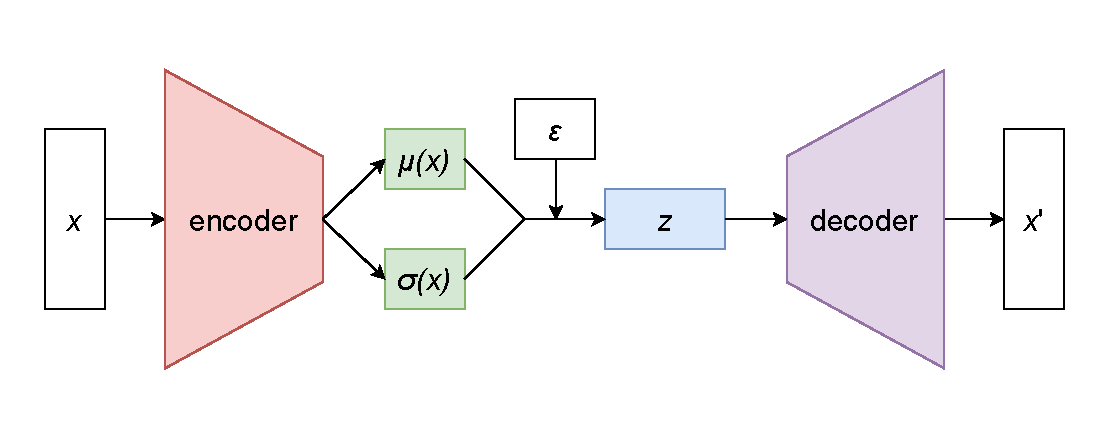
\includegraphics[width=1.0\linewidth]{images/VAE.pdf}
	\label{fig:VAE}

\noindent Our pipeline:
\begin{enumerate}
	\item Image pre-processing
	\item Features extraction: a neural network pre-trained on ImageNet produces output features.
	\item Features compression \& clustering: train a convolutional Variational Autoencoder. Learnt latent space is fed to a clustering algorithm.
\end{enumerate}



\begin{center}
	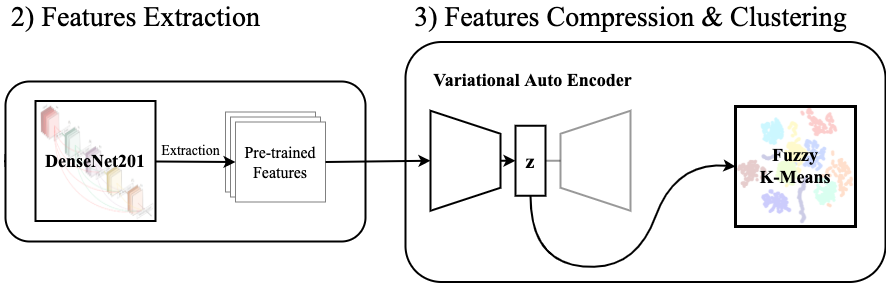
\includegraphics[width=1.0\linewidth]{images/pipeline.png}
	\label{fig:Pipeline}
\end{center}
  \vspace{0.3em}
 }





%%%%%%%%%%%%%%%%%%%%%%%%%%%%%%%%%%%%%%%%%%%%%%%%%%%%%%%%%%%%%%%%%%%%%%%%%%%%%%
%\headerbox{Poster}{name=poster,column=1,span=2,below=scholarship,above=acknowledge,ghost=yes}{
\headerbox{Datasets \& Experiments}{name=experiments,column=1,span=2, row=0,}{
%%%%%%%%%%%%%%%%%%%%%%%%%%%%%%%%%%%%%%%%%%%%%%%%%%%%%%%%%%%%%%%%%%%%%%%%%%%%%%
\begin{itemize}
	\item Lensless: 10 classes, 640 color images each.
	\item WHOI40: 40 classes, 100 grayscale images each. 
	\item WHOI22: 22 fine grained species, 300 grayscale images each.
\end{itemize}

\noindent We evaluate our pipeline with the \textit{purity} measure:
\begin{small}
	\begin{center}
		$\displaystyle \text{purity}(\Omega, C)=\frac{1}{N}\sum_k\max_j|w_k\cap c_j|$
	\end{center}
\end{small}
$\Omega=\{w_1,...,w_k\}$ set of clusters, $C=\{c_1,...,c_j\}$ set of real classes. We show qualitative and quantitative benefit using pre-trained features on the lensless dataset. 

\begin{center}
	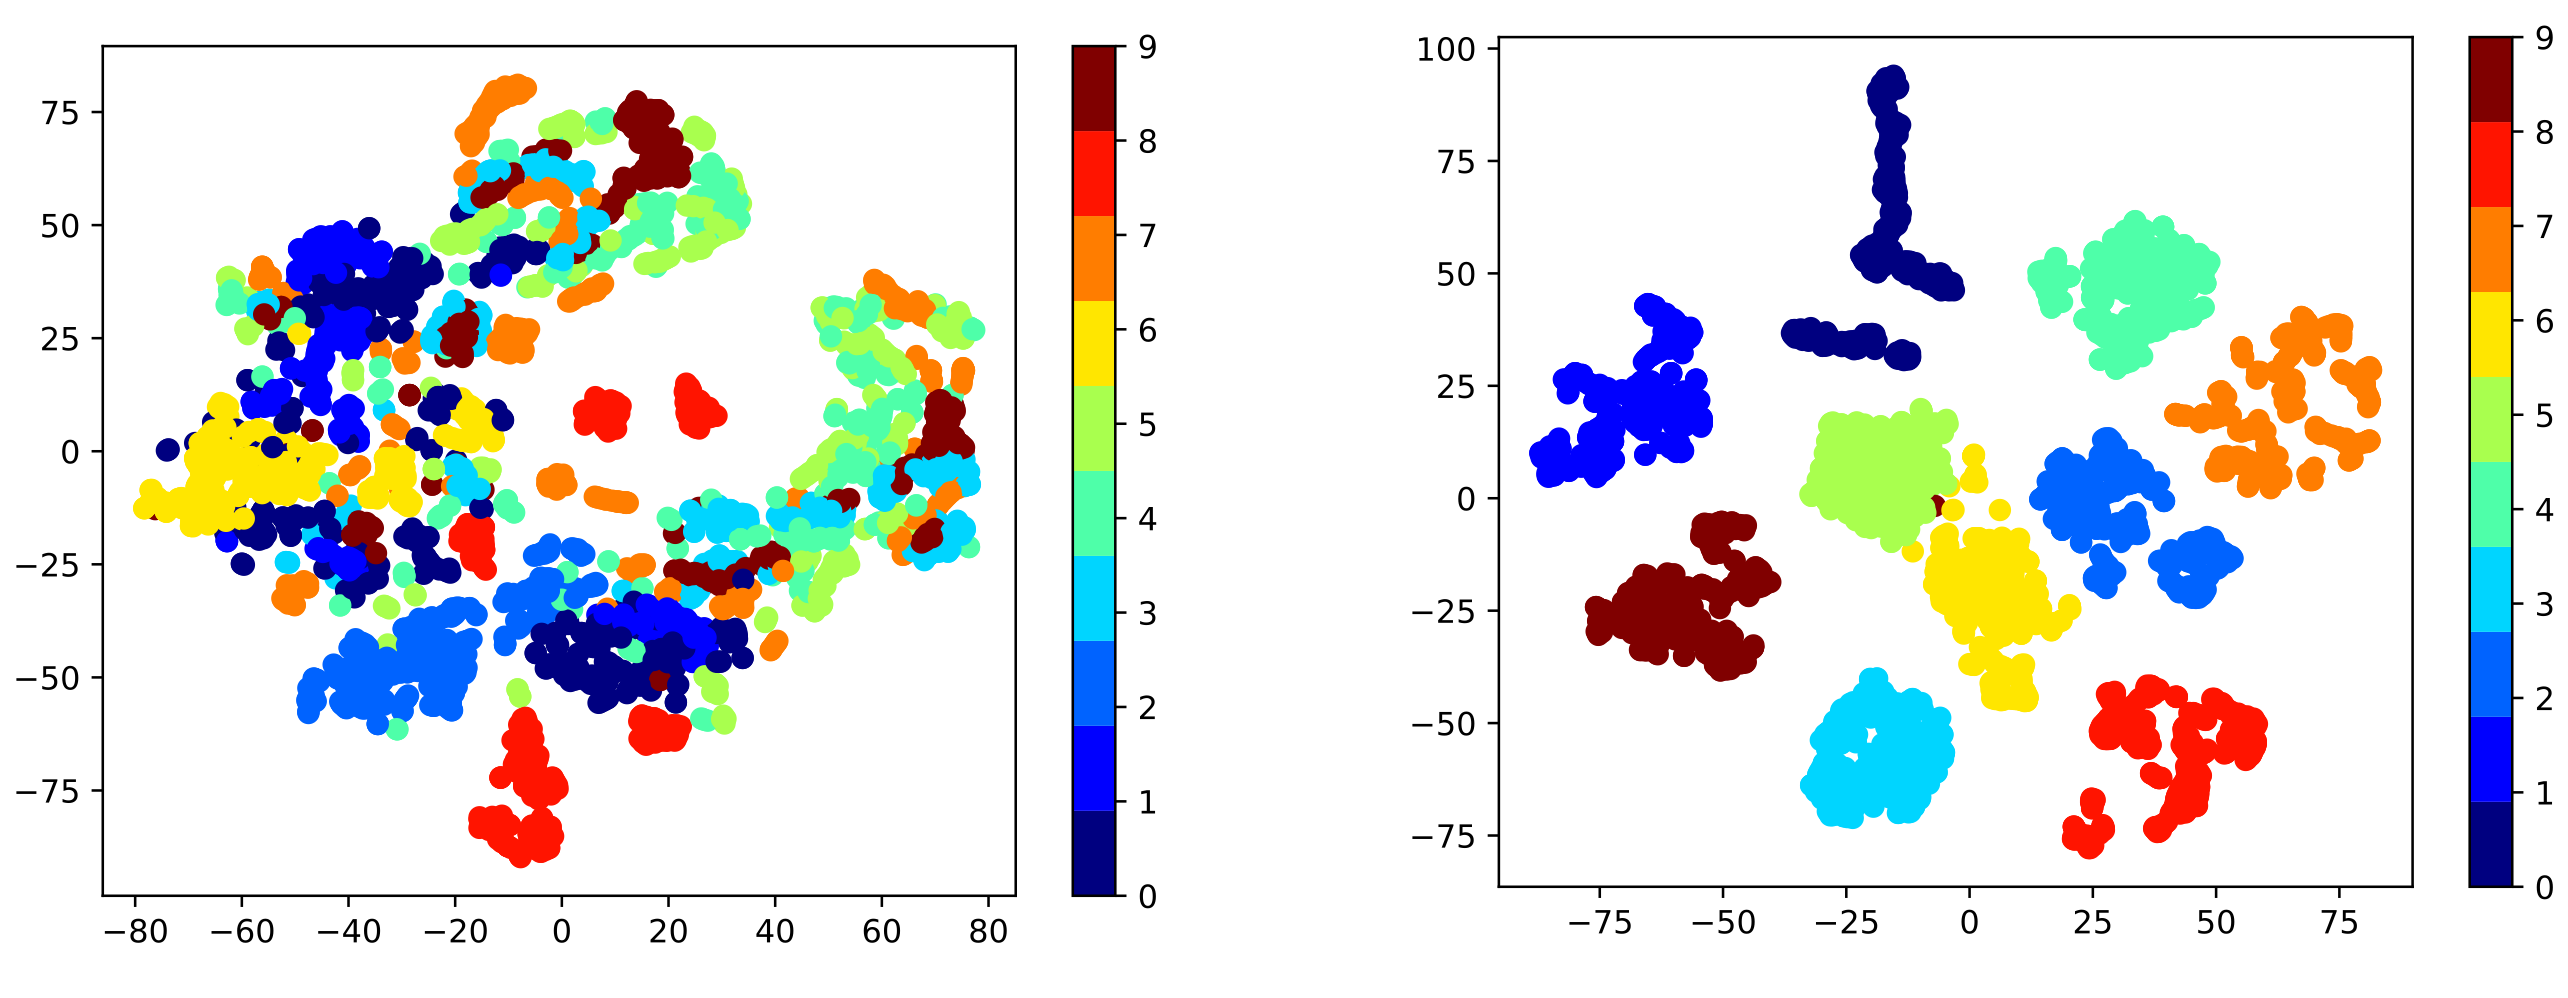
\includegraphics[width=0.6\linewidth]{images/imgs_vs_features}
	\label{fig:imgs_vs_features}
\end{center}
\begin{small}
	\begin{tabular}{ l | l l l l l }
		Algorithm/Z & 10 & 30 & 50 & 100 & 500\\
		\hline
		image-VAE & 
		\begin{tabular}{@{}l@{}} $0.53 \pm 0.017$ \end{tabular} & 
		\begin{tabular}{@{}l@{}} $0.55 \pm 0.04$ \end{tabular} & 
		\begin{tabular}{@{}l@{}} $0.58 \pm 0.01$  \end{tabular} & 
		\begin{tabular}{@{}l@{}} $0.59 \pm 0.01$ \end{tabular} & 
		\begin{tabular}{@{}l@{}} $0.62 \pm 0.01$ \end{tabular} \\
		\hline
		FE-VAE & 
		\begin{tabular}{@{}l@{}} $0.98 \pm 0.01$\end{tabular} &
		\begin{tabular}{@{}l@{}} $0.98 \pm 0.03$ \end{tabular} & 
		\begin{tabular}{@{}l@{}}$0.98 \pm 0.01$ \end{tabular} & 
		\begin{tabular}{@{}l@{}} $0.98 \pm 0.02$\end{tabular} & 
		\begin{tabular}{@{}l@{}} $0.98 \pm 0.02$\end{tabular} \\
	\end{tabular}

\begin{itemize}
	\item  Pre-trained features increases the purity by $30\%$ on average
	\item Using a bigger latent space does not imply a performance improvement
\end{itemize}
\end{small}

\noindent Quantitative results on the other datasets:

\begin{small}
\begin{tabular}{ l | l l l l l }
	Dataset/Z & 10 & 30 & 50 & 100 & 500\\
	\hline
	WHOI 40 &
	\begin{tabular}{@{}l@{}} $0.66 \pm 0.01$ \end{tabular} &
	\begin{tabular}{@{}l@{}} $0.71 \pm 0.02$ \end{tabular} &
	\begin{tabular}{@{}l@{}}$0.73 \pm 0.02$ \end{tabular} &
	\begin{tabular}{@{}l@{}} $0.77 \pm 0.01$ \end{tabular} &
	\begin{tabular}{@{}l@{}} $0.77 \pm 0.01$ \end{tabular}\\
	\hline
	WHOI 22 &
	\begin{tabular}{@{}l@{}} $0.63 \pm 0.004$ \end{tabular} & 
	\begin{tabular}{@{}l@{}} $0.66 \pm 0.01$ \end{tabular} &
	\begin{tabular}{@{}l@{}}$0.68 \pm 0.005$ \end{tabular} &
	\begin{tabular}{@{}l@{}} $0.68 \pm 0.006$ \end{tabular} &
	\begin{tabular}{@{}l@{}} $0.68 \pm 0.01$ \end{tabular} \\
\end{tabular}
\begin{itemize}
	\item Best performances correspond to a latent space size $Z=100$.
\end{itemize}
\end{small}
\noindent We compared our results with a state-of-the-art unsupervised learning pipeline.


\begin{small}
\begin{tabular}{ l | l l l l l }
	Algorithm/Dataset & Lensless & WHOI 40 & WHOI 22 \\\hline
	Pipeline from \cite{pastore}  & 0.93 & 0.71 & 0.56 \\\hline
	Ours  & \textbf{0.98} & \textbf{0.77} & \textbf{0.68} \\
\end{tabular} 
\end{small}


  \vspace{0.3em}
  }



%%%%%%%%%%%%%%%%%%%%%%%%%%%%%%%%%%%%%%%%%%%%%%%%%%%%%%%%%%%%%%%%%%%%%%%%%%%%%%
\headerbox{Conclusions}{name=conclusions,column=1,span=2, below=experiments, }{
	%%%%%%%%%%%%%%%%%%%%%%%%%%%%%%%%%%%%%%%%%%%%%%%%%%%%%%%%%%%%%%%%%%%%%%%%%%%%%%
	We introduced an efficient unsupervised pipeline for plankton images. Input images are fed to a pre-trained neural network. Output features are used as inputs to train a Variational Autoencoder. The latent space representation is used by clustering algorithm. Future developments will extend our analysis to other datasets to test our pipeline on a more general context.
	\vspace{0.5em}
}



%%%%%%%%%%%%%%%%%%%%%%%%%%%%%%%%%%%%%%%%%%%%%%%%%%%%%%%%%%%%%%%%%%%%%%%%%%%%%%
\headerbox{References}{name=references,column=1,span=2, below=conclusions}{
	%%%%%%%%%%%%%%%%%%%%%%%%%%%%%%%%%%%%%%%%%%%%%%%%%%%%%%%%%%%%%%%%%%%%%%%%%%%%%%
    \smaller
	\vspace{-0.4em}
	\bibliographystyle{ieee}
	\renewcommand{\section}[2]{\vskip 0.05em}
	\begin{thebibliography}{1}\itemsep=-0.01em
		\setlength{\baselineskip}{0.4em}
		\bibitem{boyce}
		Boyce, D et al. Global phytoplankton decline over the past century, in \textit{Nature 466}, 2010
		\bibitem{diederik}
		Diederik, K et al. Auto-Encoding Variational Bayes, in \textit{arXiv}:1312.6114, 2014
		\bibitem{pastore}
		Pastore, V et al. Annotation-free learning of plankton for classification and anomaly detection, in \textit{Scientific Reports 10}, 2020

	\end{thebibliography}
	\vspace{0.3em}
}



\end{poster}

\end{document}
